\documentclass{article}
\usepackage{ctex}
\usepackage{amsmath}
\usepackage{graphicx}
\usepackage{wrapfig}
\usepackage{caption}
\usepackage[top=0.8in, bottom=0.8in,left=0.8in, right=0.8in]{geometry}
\usepackage{float} 
\usepackage{subfigure}
\usepackage{subcaption}
\usepackage{bm}
\xeCJKsetup{CJKmath=true} 
\begin{document}
\section*{匀强磁场中带电小球在圆盘上的运动(50分)}
\begin{wrapfigure}{r}{7cm}
	\vspace{-15pt}    % 对应高度1
	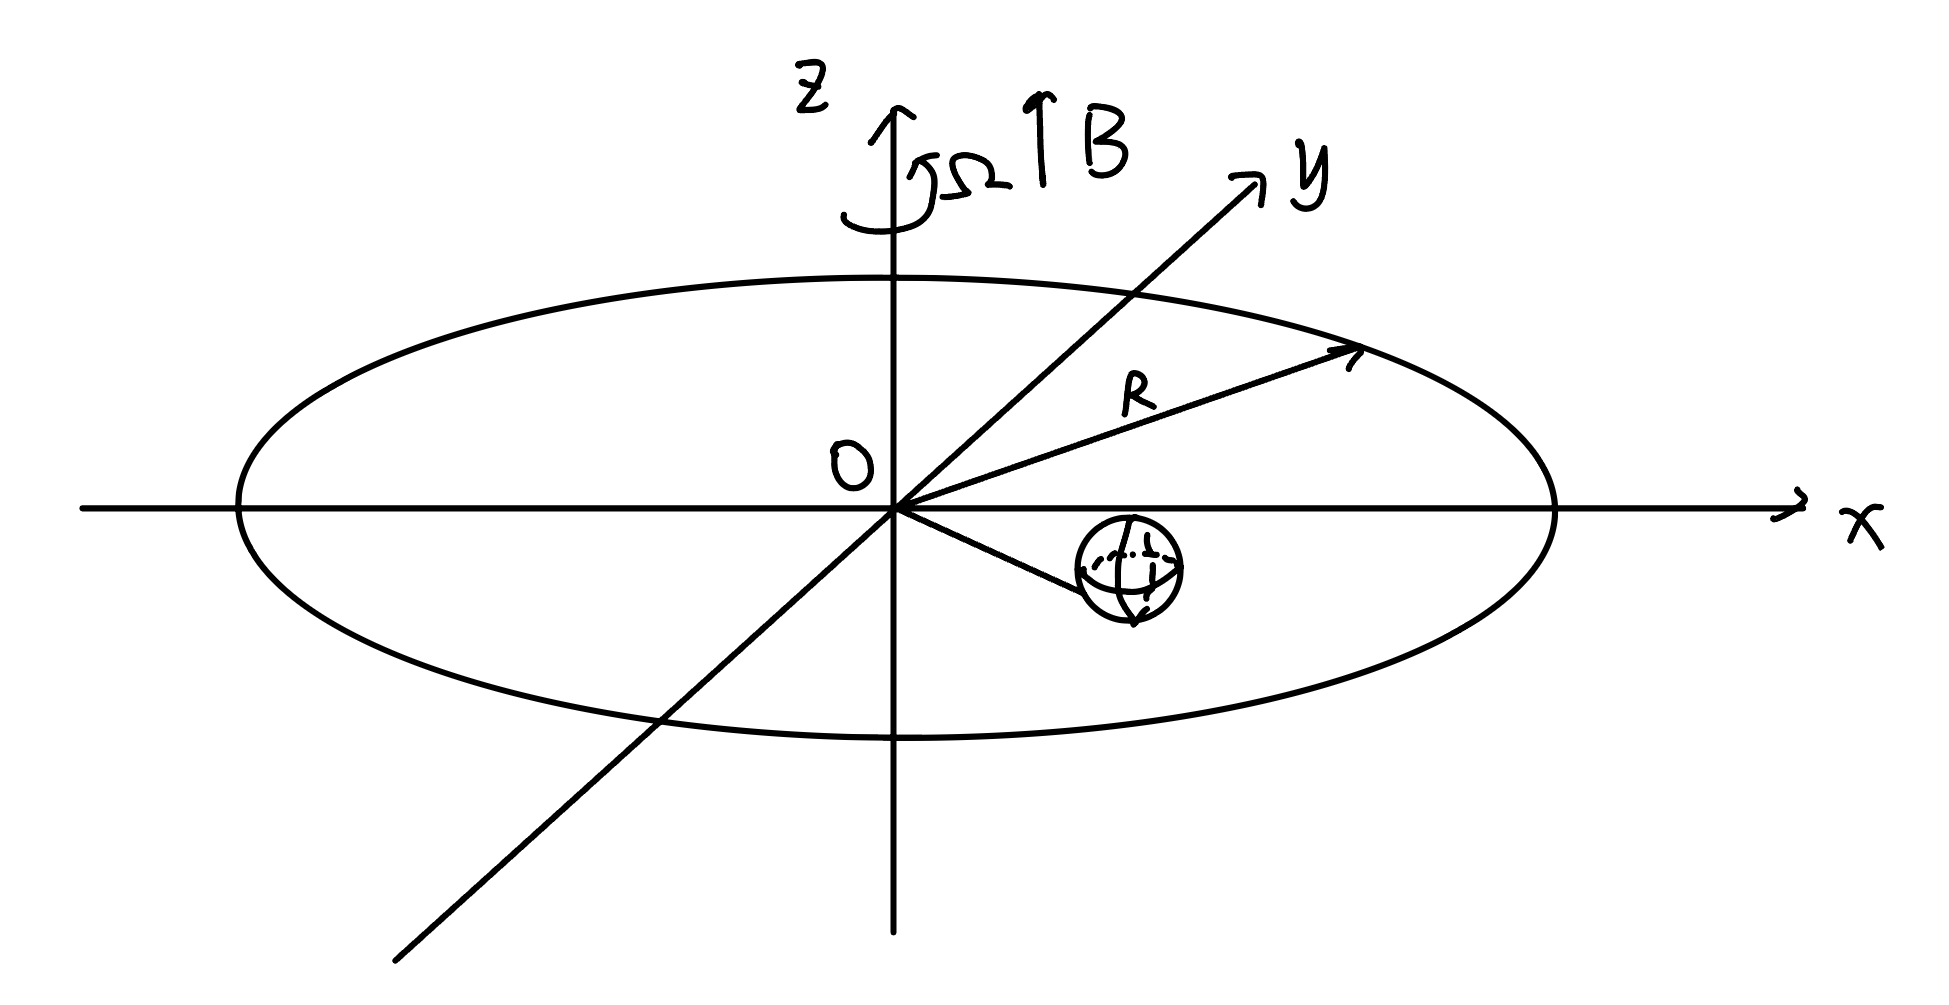
\includegraphics[width=7cm]{img/0002.1.jpeg}\\
	\vspace{-15pt}    % 对应高度2
	\caption{}
	\vspace{-15pt}    % 对应高度3
\end{wrapfigure}
考虑一个沿$z$轴以匀角速度$\Omega$转动的薄圆盘半径为$R$,质量为$M$。有一半径为$r$,均匀带电量为$Q$,质量为$m$的小球,小球与圆盘间无滑动。全空间存在竖直向上的匀强磁场,大小为$B$.\par
初始将小球静止放在$(r_0,0,0)$处,考虑其运动。\par
\begin{itemize}
\item[(1)]当带电小球以$\vec{\omega}$转动时,求带电小球的总磁矩$\vec{\mu}$。\par
注:磁矩定义$\vec{\mu}=I\vec{S}$\par
\item[(2)]初始$t=0$,求解之后的运动。
\end{itemize}
\end{document}